The outcome of your model is determined by the parameter settings that you chose. Parameter values may have been estimated from your own empirical data, from first principles, from tradition, from literature, from expert knowledge (with the prime expert often, conveniently, being yourself), or from more or less well founded guesswork. However you arrived at the parameter values, they are commonly summarised in one value, namely the expected mean value. But when you think more carefully about it, you will often realise that this is a gross simplication of the real uncertainty, in which many parameters are shrouded. 

Parameter values may be uncertain for many reasons. Customarily the uncertainty of an average is measured by its standard error. The underlying reason for this uncertainty could be sampling noise; if you sampled the whole population you would know the true mean with certainty. However, other, irreducible reasons for uncertainty are plentiful. For instance, the temperature of an insect depends on where it chooses to sit; hence the average temperature of all insects in a population will change with factors and processes that you likely have not got the resources, nor the interest, to model in detail. 

In both \concept{uncertainty analysis} and \concept{sensitivity analysis}, you specify model parameters by their estimated distribution (\eg\ uniform or normal), rather than their estimated mean. Thus for a uniform distribution you would supply the minimum and maximum value -- and for a normal distribution, its mean and standard deviation. In uncertainty analysis, you proceed to analyse the uncertainty in model outcomes resulting from the uncertainty in model parameters. In sensitivity analysis, you seek to explain the uncertainty in model outcomes by the model parameters, answering the question: Which model parameters are mostly responsible for the uncertainty in model outcomes?

In both uncertainty analysis and sensitivity analysis, you specify model parameters (\ie\ inputs) by their estimated distribution (\eg\ uniform or normal), rather than their estimated mean. Thus for a uniform distribution you would supply the minimum and maximum value and for a normal distribution, its mean and standard deviation. In \concept{uncertainty analysis}, your aim it to analyse the uncertainty in model outcomes resulting from the uncertainty in model parameters. In \concept{sensitivity analysis}, you seek to explain the uncertainty in model outcomes answering the question: Which model parameters are mostly responsible for the uncertainty in model outcomes?

\section{Setting up the input distributions}
In general you may consider some model parameters certain enough to be specified simply by their estimated mean value. If so then only a subset of the model parameters will need to be specified by their distribution. The model obviuously needs to run many times to ascertain the distribution of its outcomes. You set the number of runs by the \code{simulations} input to the \code{Simulation} box. Before each iteration, the \code{reset} method of all boxes is called once before the ensuing repeated calls of the \code{update} for all boxes. The number of times all boxes are updated is determined by the \code{steps} input to the \code{Simulation} box.

\begin{figure} [hb]
\centering
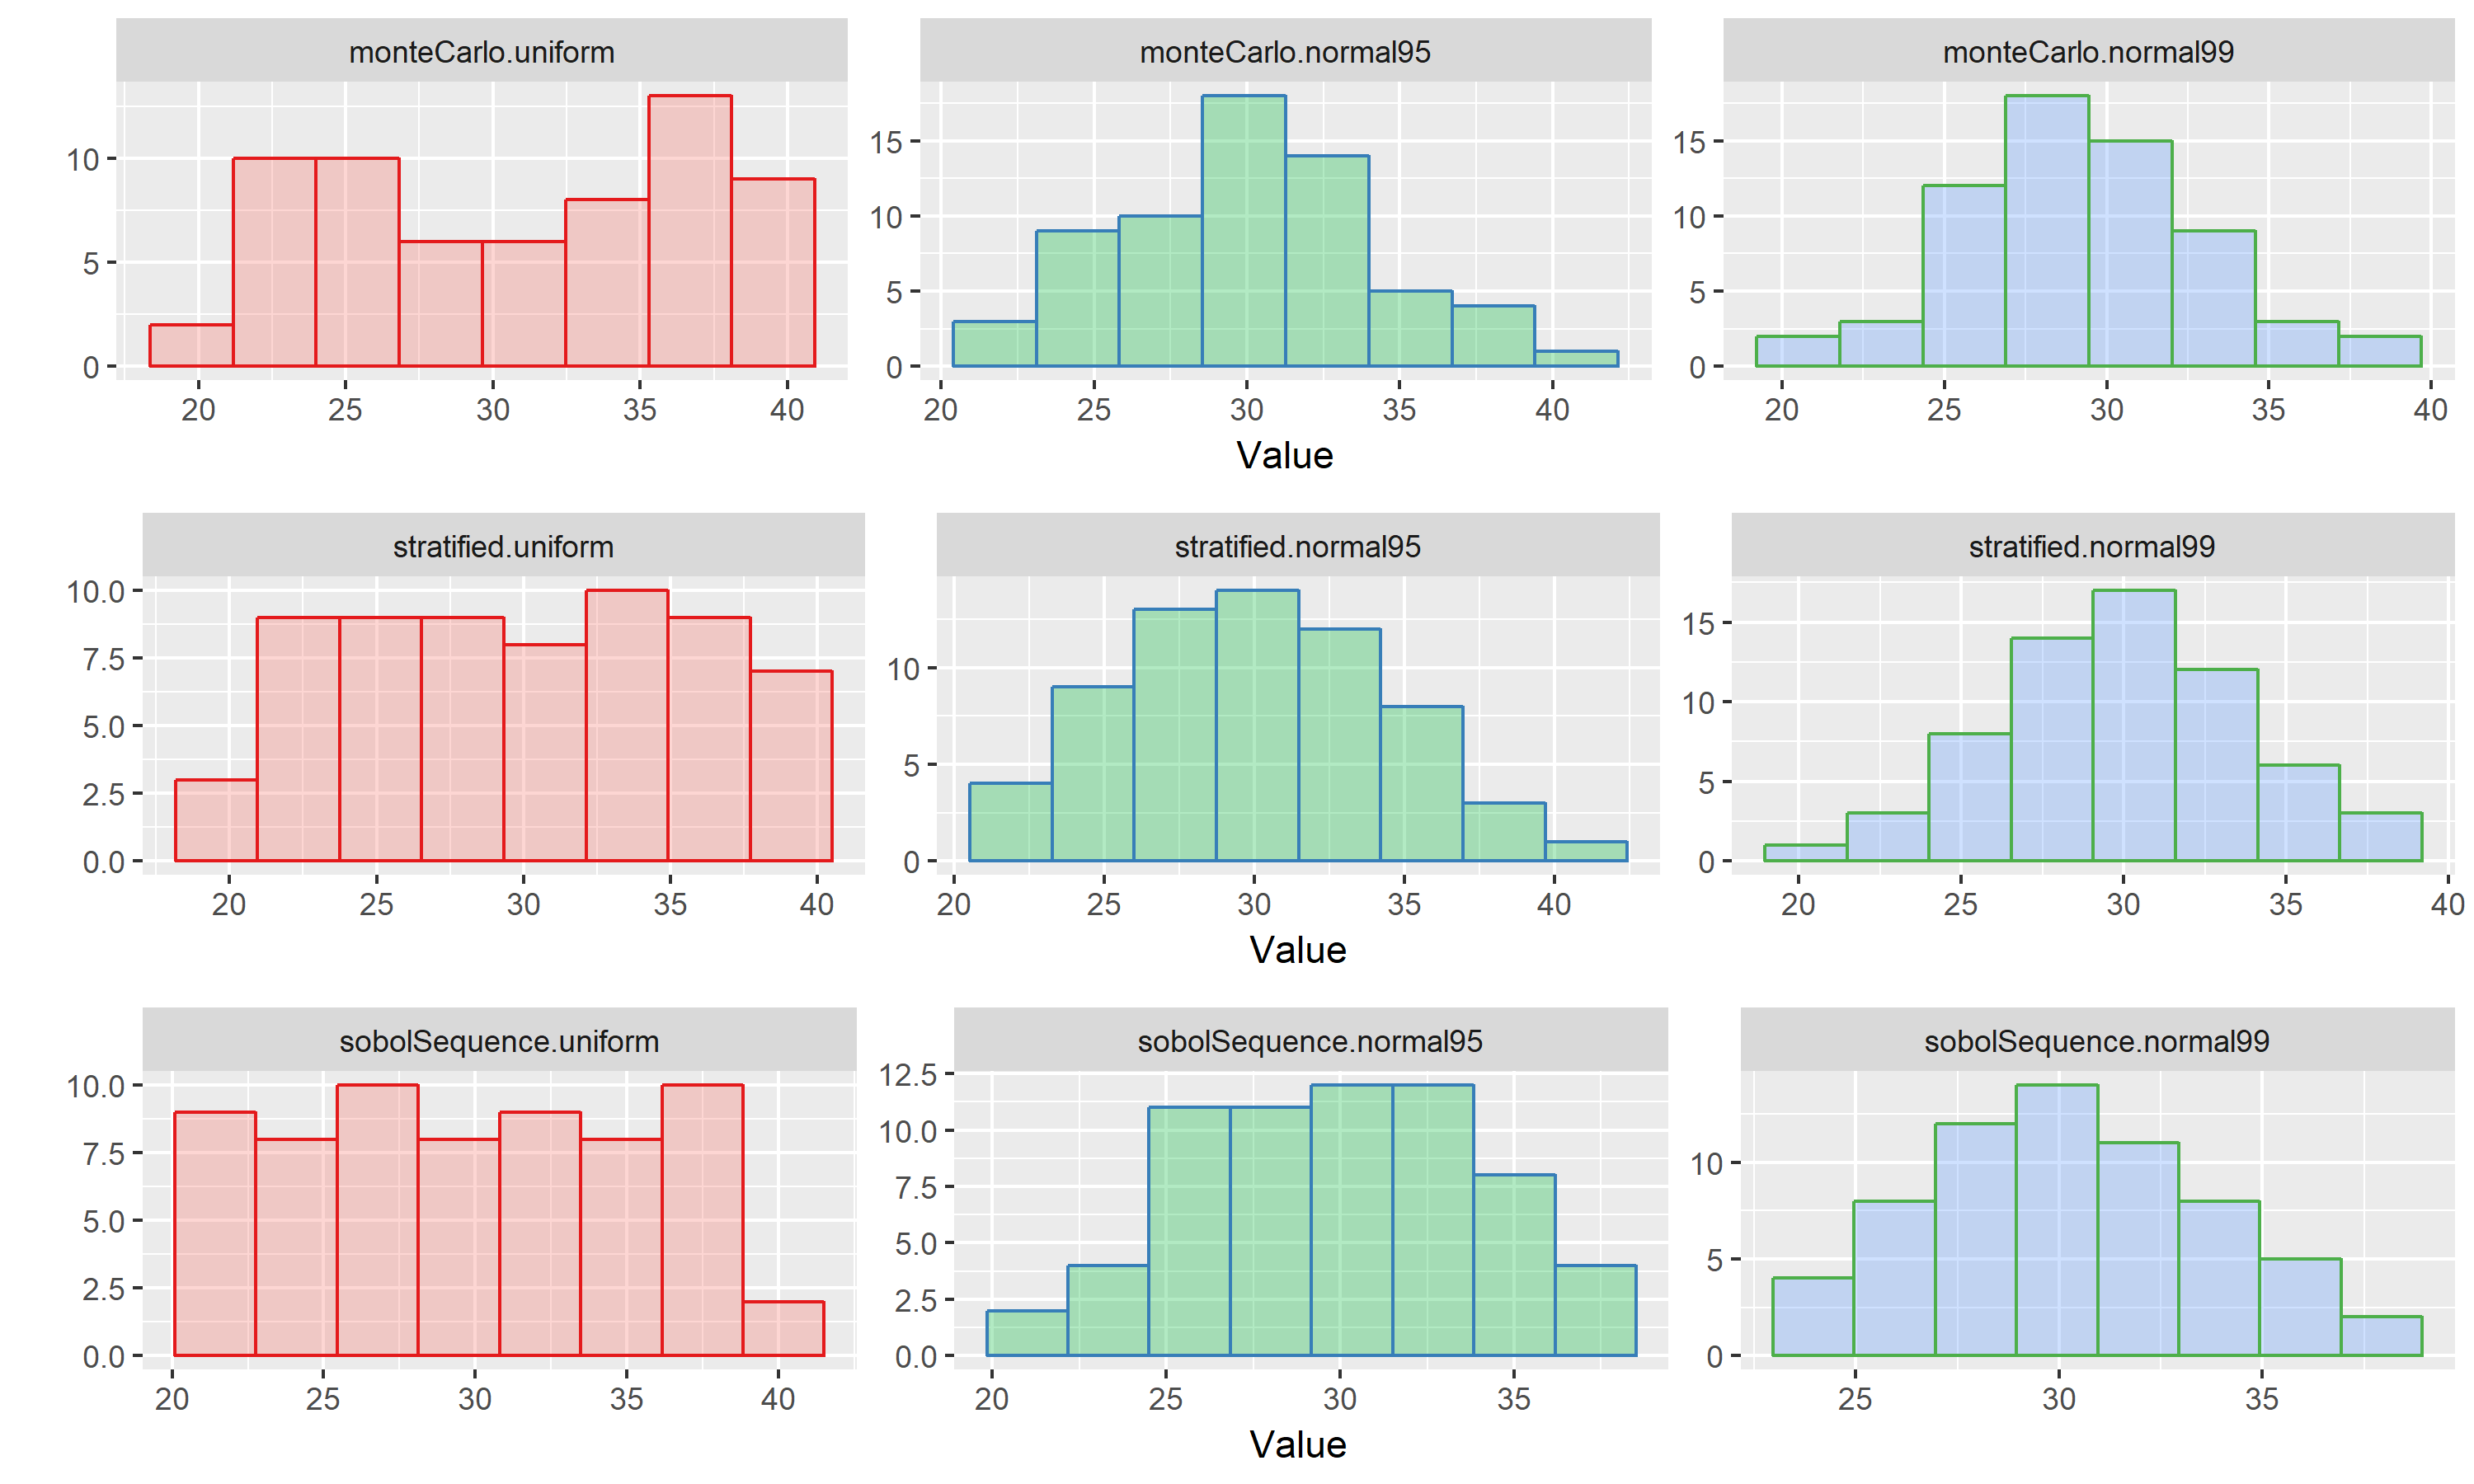
\includegraphics[width=\textwidth]{graphics/uncertainty-analysis-set-up}
\caption{Parameter distributions produced by the \filename{\inputfolder/book/uncertainty-analysis-set-up.box} script.}
\label{fig:uncertainty-analysis-set-up}
\end{figure}

In \iref{fig:uncertainty-analysis-set-up} you can see examples of some of the input distributions supported by \US. The complete list of distributions is defined by the boxes classes available for random variables:
\begin{itemize}
\item \codenobox{RandomBinomial}
\item \codenobox{RandomLognormal}
\item \codenobox{RandomNormal}
\item \codenobox{RandomUniform}
\item \codenobox{RandomUniformInt}
\end{itemize}
It may come as a surprise but all distributions, except for the binomial, are specified by their minimum and maximum values. For the distributions that are born limitless (log and lognormal), the minimum and maximum values delimit the central 95\% of the distribution. So, for example, a normal distribution with min-max limits of 20-40 will have a mean value of 30. Likewise, a lognormal distribution with a min-max of 10-1000 will have a mean of 100. The standard deviation will be calculated to match the central 95\% (default value, see below) inside the min-max limits which are set by the \code{min} and \code{max} inputs.

For the binomial, normal and lognormal distributions, an additional input \code{P} specifies the probability for a positive (true) binomial outcome (default \code{P}=0.5), or else the central proportion (default \code{P}=0.95) of the distribution inside the min-max limits.

All min-max intervals are closed-open meaning that the min value is included and the max value is excluded from the interval. However, for the \code{RandomUniformInt}, which produces integer values in the min-max interval, the interval is closed-closed, \ie\ the max value is included in the distribution.

\US\ provides three methods of generating random numbers from any of the distributions above. They are defined by these three box classes:
\begin{itemize}
\item \codenobox{RandomiserMonteCarlo}
\item \codenobox{RandomiserStratified}
\item \codenobox{RandomiserSobolSequence}
\end{itemize}
If the simulation is running for $N$ iterations (defined by the \code{iterations} input to the \code{Simulation} box) then the Monte Carlo randomiser will pick a value at random $N$ times within the desired distribution. The stratified method will first slice the distribution into $N$ slices of equal area and then for each iteration pick a slice at random (without replacement, \ie\ each slice will be picked only once) and then pick a random number inside that slice. Compared to the Monte Carlo method, this will make the resulting distribution resemble more closely the population sampled from.

The Sobol' sequence differs from the others in that it is not truely random. You will get the same sequence of numbers every time you invoke it! Whereas the previous two methods produce pseudo-random numbers, the Sobol' sequence is said to consist of quasi-random numbers. However, if you have more than one random parameter for your model (most likely, you will), the Sobol' sequence ensures a maximum spread of numbers in the multi-dimensional space defined by the min-max limits for each of your model parameters. This means that the distribution of your model outcomes will converge more quickly, \ie\ you need a lower $N$ for conversion which will save you execution time. Due to the working of Sobol' sequences, $N$ must be a power of 2, $N=2^n$. You will get an error message at the \US\ prompt if you break this rule.

If you revisit \iref{fig:uncertainty-analysis-set-up}, you will now realise that each row of  distributions is generated by one of the three randomisers. Each column exemplifies a certain distribution: uniform, normal with 95\% coverage and normal with 99\% coverage. All distributions span the same 20-40 interval.

The Monte Carlo method (\iref{fig:uncertainty-analysis-set-up} top row) yields the most noisy distribution as expected. A total of $N=64$ iterations were chosen (line 3 below), so in the uniform distribution, 8 hits are expected on average in each of the 8 bins defined by the histogram. 

If you compare the 95\% and 99\% normal distributions you will notice that at \code{P}=99\%, the peak is more pronounced. This central tendency will increase with increasing \code{P}.

If we could visualise the joint three-dimensional distribution of each row of distributions (these individual distributions are known as marginal distributions) then we would see that the Sobol' sequence were best at dispersing its sampling throughout that space.

The script generating \iref{fig:uncertainty-analysis-set-up} is straightforward, although it should be noted that when random numbers are used as input to a model, they should all be generated by the same randomiser (Monte Carlo, stratified or Sobol' sequence). Here they were mixed only to demonstrate their differences:

\lstset{numbers=left}
\begin{boxscript}
// uncertainty-analysis-set-up.box
Simulation sim {
  .iterations = 64
  .steps = 1
  .silent = TRUE
  Box monteCarlo {
    RandomiserMonteCarlo randomiser {
    }
    RandomUniform uniform {
      .min = 20
      .max = 40
    }
    RandomNormal normal95 {
      .min = 20
      .max = 40
    }
    RandomNormal normal99 {
      .min = 20
      .max = 40
      .P = 0.99
    }
  }
  Box stratified {
    RandomiserStratified randomiser {
    }
    RandomUniform uniform {
      .min = 20
      .max = 40
    }
    RandomNormal normal95 {
      .min = 20
      .max = 40
    }
    RandomNormal normal99 {
      .min = 20
      .max = 40
      .P = 0.99
    }
  }
  Box sobolSequence {
    RandomiserSobolSequence randomiser {
    }
    RandomUniform uniform {
      .min = 20
      .max = 40
    }
    RandomNormal normal95 {
      .min = 20
      .max = 40
    }
    RandomNormal normal99 {
      .min = 20
      .max = 40
      .P = 0.99
    }
  }
  OutputR {
    PageR {
      .width = 8
      .height = 6
      PlotR {
        .ports = monteCarlo/*[value]|end
        .geom = "histogram(8)"
        .ncol = 3
      }
      PlotR {
        .ports = stratified/*[value]|end
        .geom = "histogram(8)"
        .ncol = 3
      }
      PlotR {
        .ports = sobolSequence/*[value]|end
        .geom = "histogram(8)"
        .ncol = 3
      }
    }
  }
}
\end{boxscript}
\lstset{numbers=none}

In general you define all the random inputs inside one box, as exemplified in lines 6-22. Most often it is most natural to call this box simply \code{random}. In this special case, it was called \code{monteCarlo} as we are comparing different randomisation methods. The first box  inside (lines 7-8) should be one of the three randomiser boxes: \code{RandomiserMonteCarlo}, \code{RandomiserStratified} or \code{RandomiserSobolSequence}. Then follows one box of the \code{Random} family for each random input (lines 9-21).

In this box script, the random values were not put to any use as inputs to a proper model. They are simple shown in the output (lines 62, 67 and 72). Note the used of the \code{|end} filter which assures that we plot only the final value of each input. They change value only at the beginning of each iteration, which in this case last only one step (line 4).  

\section{Uncertainty analysis}
We will use a predator-prey model (\filename{\inputfolder/book/func-resp/func-resp-pred-prey.box}) as an object for uncertainty analysis. The script contains the original code extended with random inputs (lines 6-29) and some adjusted outputs (lines 43-62) :

\lstset{numbers=left}
\begin{boxscript}
// uncertainty-analysis-pred-prey.box
Simulation sim {
  .iterations = 128
  .steps = 365
  .silent = TRUE
  Box random {
    RandomiserSobolSequence randomiser {
    }
    RandomUniform attackRate {
      .min = 0.1
      .max = 1
    }
    RandomNormal conversionCost {
      .min = 0.24
      .max = 0.26
    }
    RandomUniform k {
      .min = 10
      .max = 40
    }
    RandomUniform fecundityButterfly {
      .min = 20
      .max = 80
    }
    RandomUniform fecundityPredator {
      .min = 30
      .max = 50
    }
  }
  :
  Box butterfly {
  :
      Stage oviposition {
        .inflow = ../preOviposition[outflow]
        .duration = 10
        .timeStep = 1
        .growthFactor = random/fecundityButterfly[value]
        .k = random/k[value]
      }
  :
  }
  :
  OutputR {
    PageR {
      .xAxis = random/*[value]
      .width = 10
      .height = 4
      PlotR {
        .ports = */egg[content]|end
        .ggplot = "geom_smooth(colour='yellow')"
      }
    }
    PageR {
      .width = 6
      .height = 3
      PlotR {
        .ports = */egg[content]|end
        .type = "histogram(10)"
        .ncol = 5
      }
    }
  }
}
\end{boxscript}
\lstset{numbers=none}

The random inputs include the highly uncertain attack rate of the functional response (lines 9-12), a very certain energy budget parameter (lines 13-16), the dispersion parameter ($k$) of the distributed delay used in all \code{Stage} boxes (lines 17-20), and butterfly and and predator fecundities (lines 21-28).

The random values are used as inputs in the predator-prey model. Only two examples are included here, showing how to apply random butterfly fecundity (line 37) and \code{k} (line 38).

As response variables of the model, we chose final egg numbers (lines 49 and 57). These are the eggs going into hibernation at the end of the year. Two plots are produced by the script. The first one (\iref{fig:uncertainty-analysis-pred-prey-1}) has the random parameter on the \xaxis\ and the response variable on the \yaxis\ (lines 44-52). The default plot shows one point for each iteration (128 points in total, \cf\ line 3) on top of which have been added a trend curve (line 50). 

\begin{figure} 
\centering
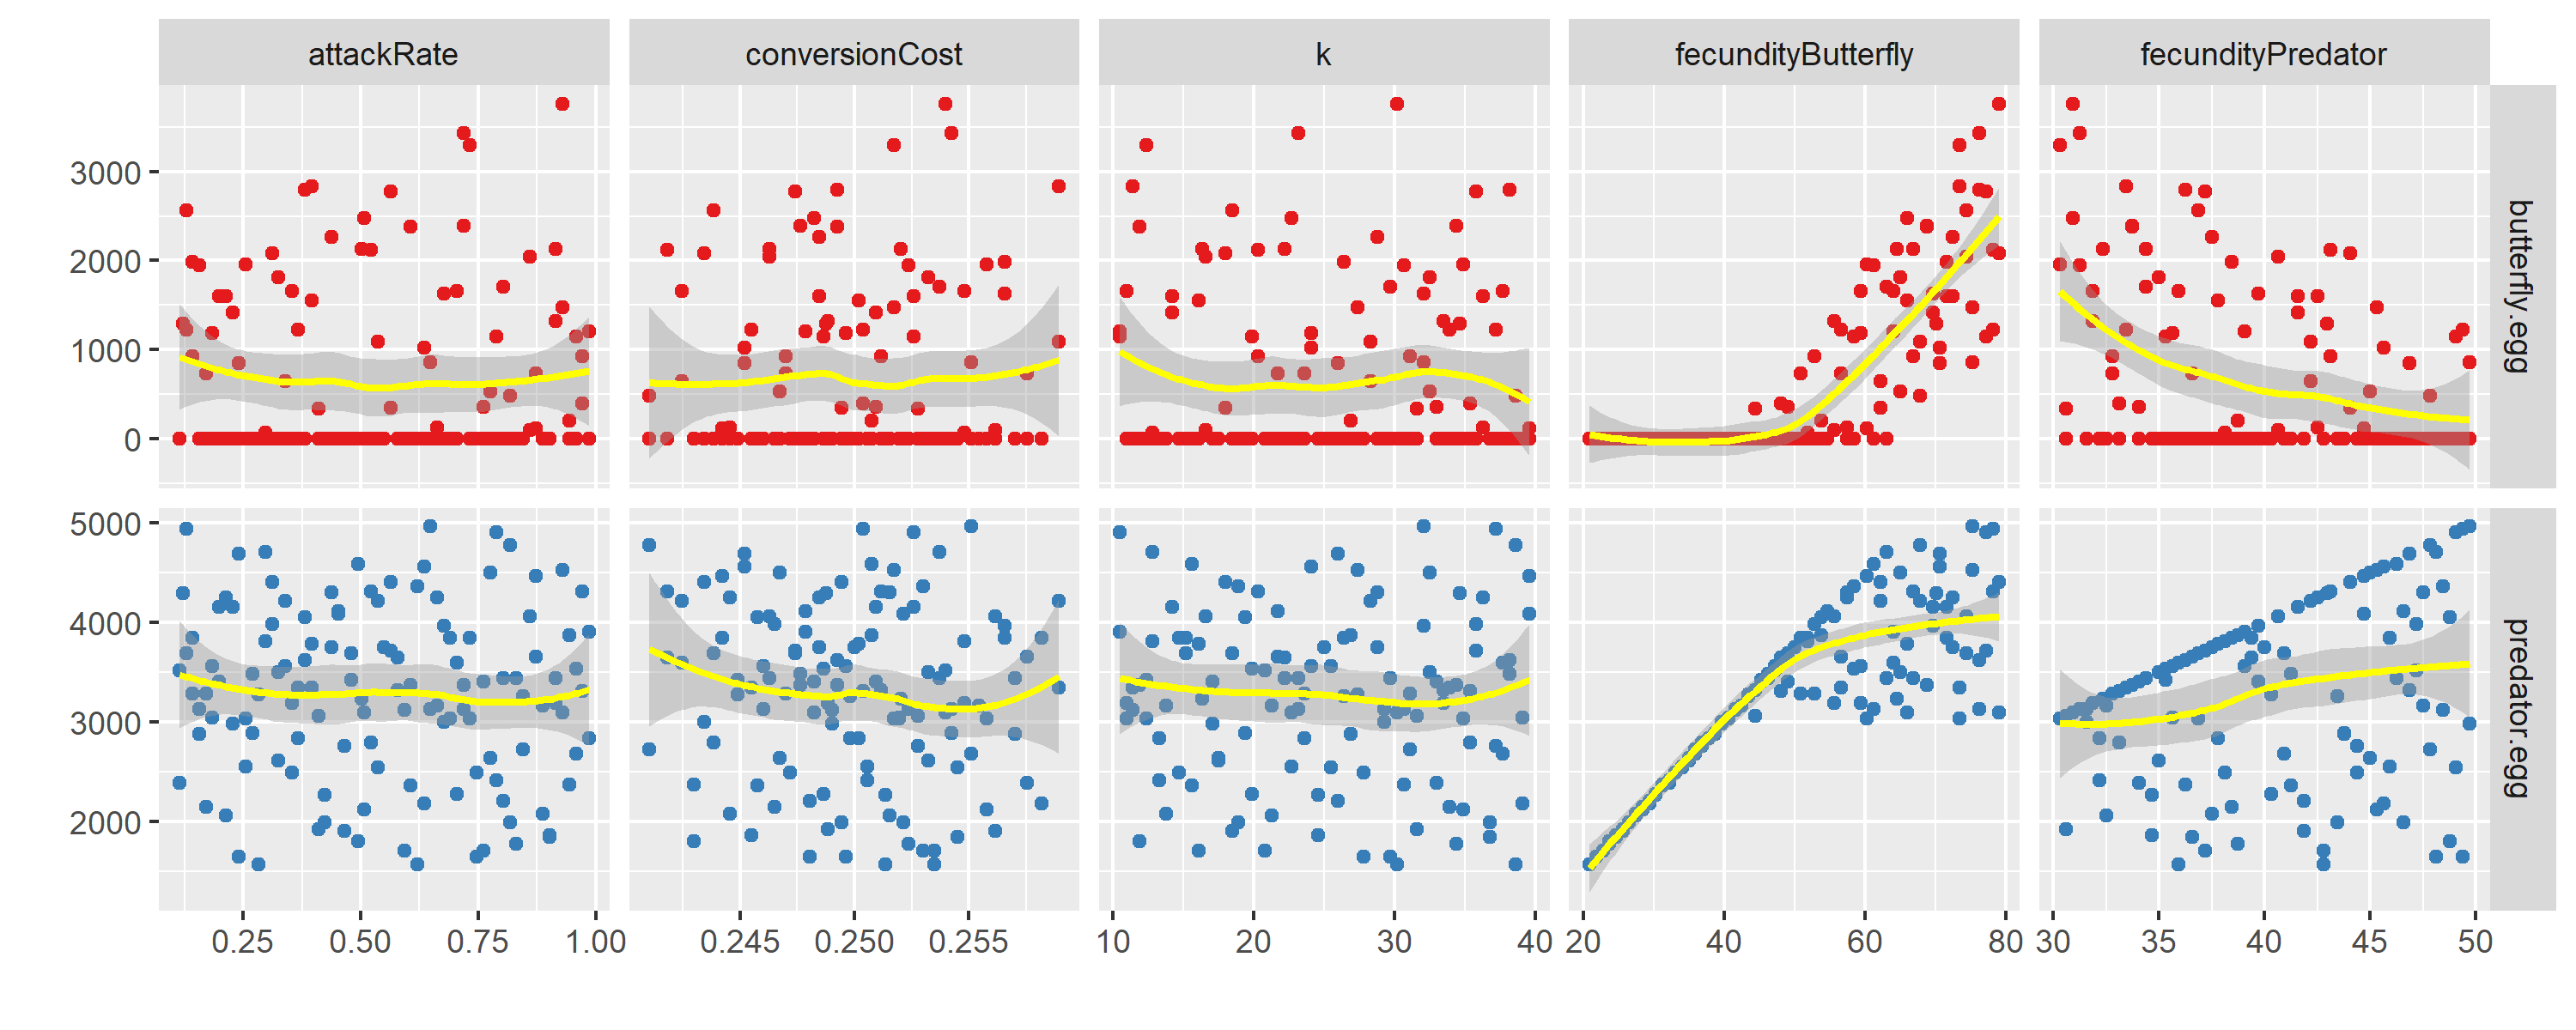
\includegraphics[width=\textwidth]{graphics/uncertainty-analysis-pred-prey-1}
\caption{The impact of five model inputs on two model outputs. Produced by the \filename{\inputfolder/book/uncertainty-analysis-pred-prey.box} script.}
\label{fig:uncertainty-analysis-pred-prey-1}
\end{figure}

The immediate impression is that the final density of butterfly eggs increased with butterfly fecundity and decreased with predator fecundity --- and \viceversa\ for the final density of predator eggs. Surpringly, there was no clear response to attack rate, even though it was allowed to vary over a large range to reflect its uncertainty. Remember that these plots show only the marginal effect of each input; any interactions are hidden.

The other plot (\iref{fig:uncertainty-analysis-pred-prey-2}) produced by lines 53-61 shows the  distribution of both model outcomes. For the butterfly the distribution is long-tailed with a predominance of very low numbers. From \iref{fig:uncertainty-analysis-pred-prey-1} we already knew that a lot of them are zeroes; the butterfly population was eradicated. The predator population is doing fine in all cases --- at least for one year.

\begin{figure} 
\centering
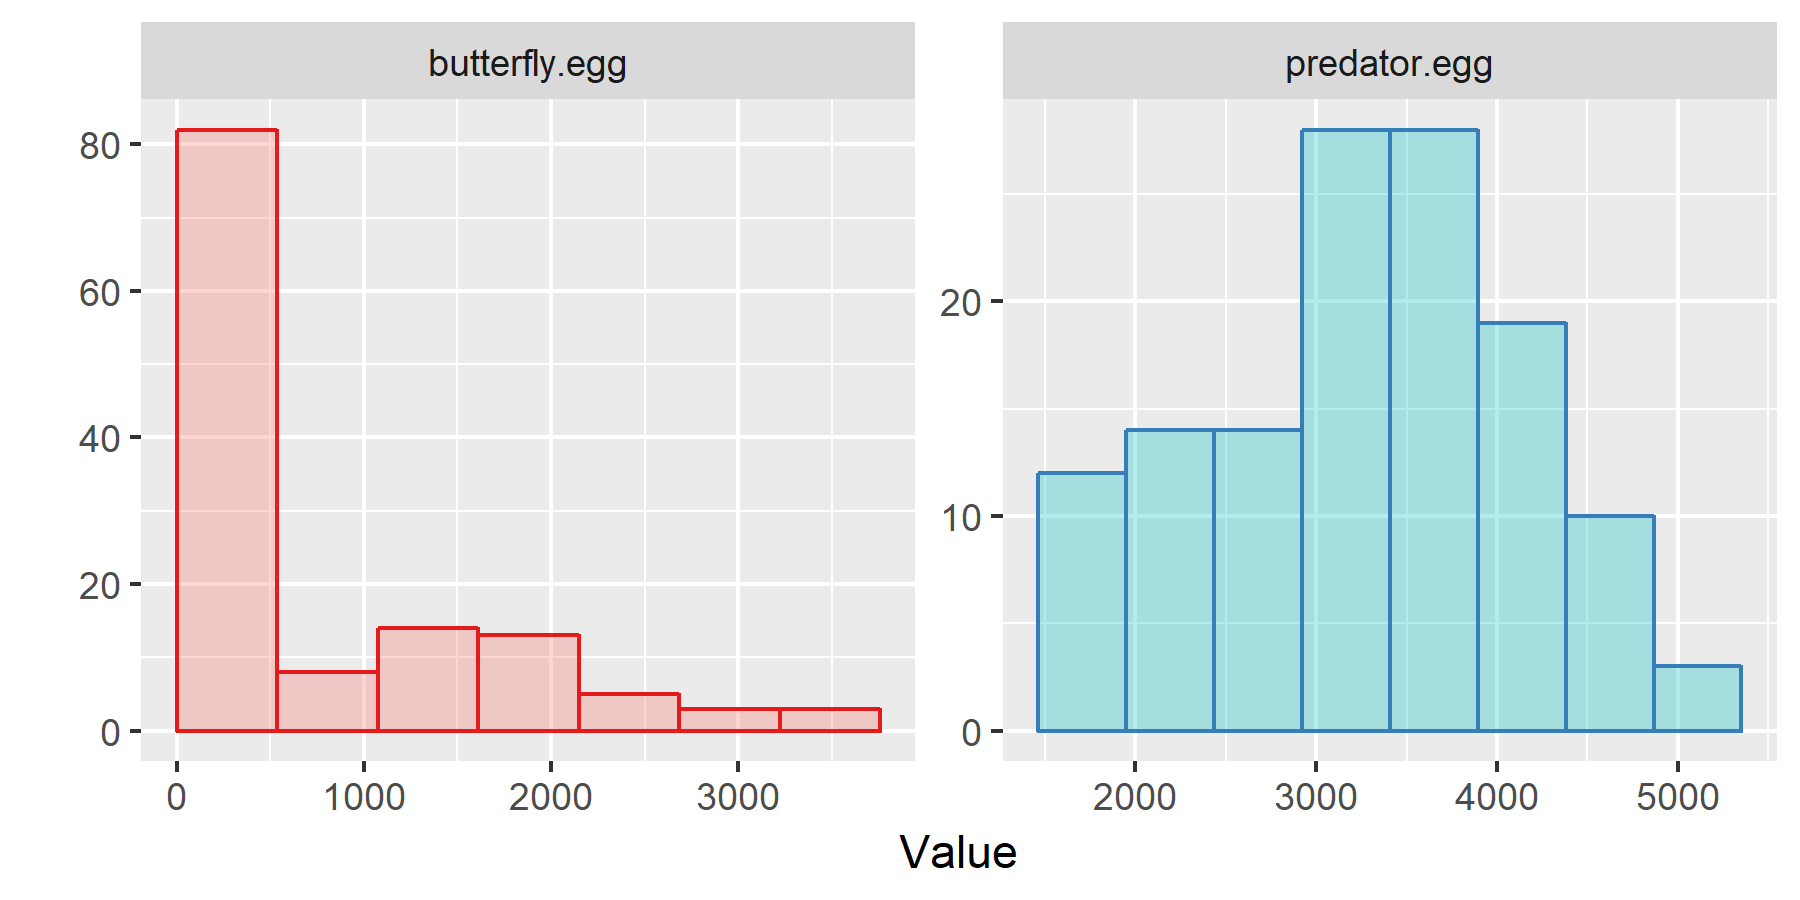
\includegraphics[width=\textwidth]{graphics/uncertainty-analysis-pred-prey-2}
\caption{The distribution of two model outputs illustrating model uncertainty. Produced by the \filename{\inputfolder/book/uncertainty-analysis-pred-prey.box} script.}
\label{fig:uncertainty-analysis-pred-prey-2}
\end{figure}

\FloatBarrier
\section{Sensitivity analysis}
The sensitivity analysis carried out by \US\ is a so-called \concept{global sensitivity analysis} in which all uncertain inputs are varied simultaneously, not just one at a time. The analysis result in \concept{Sobol' indices} \citep[][page~164-167]{Saltelli08} which indicate the sensitivity of model outcomes to uncertainty in each of the model inputs.

You need to change only little in the \filename{\inputfolder/book/uncertainty-analysis-pred-prey.box} script to add sensitivity analysis to the uncertainty analysis:

\lstset{numbers=left}
\begin{boxscript}
// sensitivity-analysis-pred-prey.box
Simulation sim {
  .iterations = 224 
  .steps = 365
  .silent = TRUE
  Box random {
    RandomiserSobolSequence randomiser {
      .doSensitivityAnalysis = TRUE
      .bootstrapSize = 1000
    }
  :
  }
  :
  OutputR {
    :
    PageR {
      .xAxis = random/*[value]
      .width = 10
      .height = 4
      PlotR {
        .ports = */egg[content]|end
        .type = "SobolConvergence"
        .fontSize = 11
      }
    }
    PageR {
      .xAxis = random/*[value]
      .width = 5
      .height = 7
      PlotR {
        .ports = */egg[content]|end
        .type = "SobolIndices"
      }
    }
  }
}
\end{boxscript}
\lstset{numbers=none}

First of all, you need too set the \code{doSensitivityAnalysis} flag to \code{TRUE} (line 8). The \code{bootstrapSize} input (line 9) is used to calculate confidence limits for the Sobol' indices. The post-processing time in R (after the simulation has finished in \US) will increase with increasing \code{bootstrapSize} but not dramatically. A common size in literature is 10,000. Here, we chose a value of 1000 for a quicker demonstration.

When you run the model, you will receive an error message if the \code{iterations} (line 3) have not been set properly according to the requirements of the randomiser. The number of iterations must equal $(2+k)N$ where $k$ is the number of inputs being analysed (we've got $k=5$) and $N$ is the so-called sample size. In this case, where the randomiser is a \code{RandomiserSobolSequence}, there is the further constraint that $N$ must be a power of 2, $N=2^n$. Here we chose $(2+5)32=224$ iterations.

With \code{doSensitivityAnalysis = TRUE} you can still get the same output as we saw for uncertainty analysis (\iref{fig:uncertainty-analysis-pred-prey-1}), but with sensitivity analysis two additional plots have become available, both dealing with the Sobol' indices. In these plots the \code{xAxis} inputs (lines 17 and 27) stands for the uncertain inputs to the model, while the \code{ports} lines (21 and 31) are the outputs of the model undergoing sensitivity analysis.

\begin{figure} 
\centering
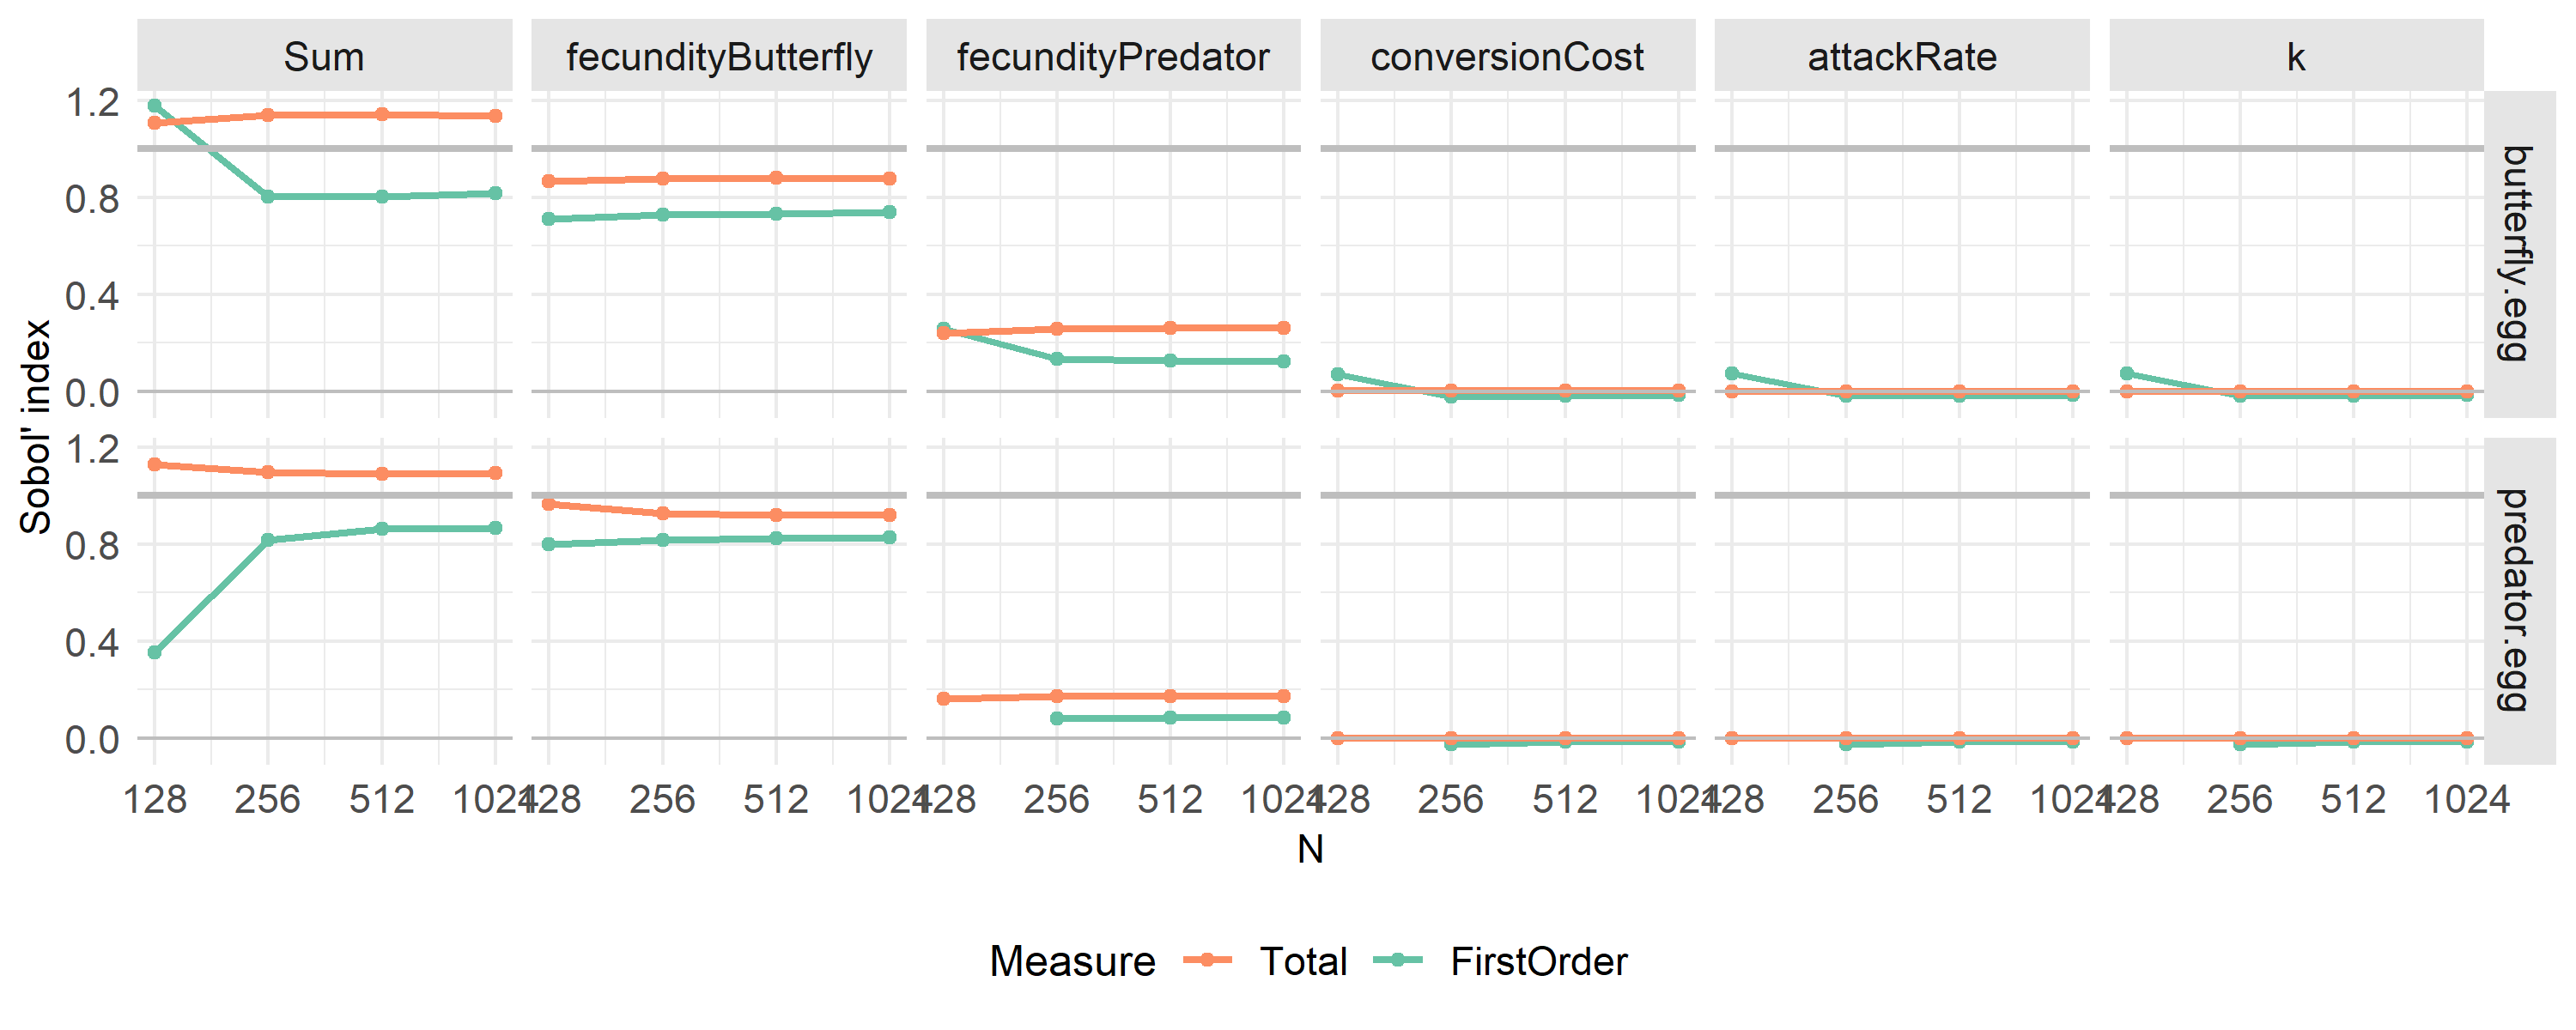
\includegraphics[width=\textwidth]{graphics/sensitivity-analysis-pred-prey-2}
\caption{Convergence of Sobol' indices with increasing sample size ($N$) produced by the \filename{\inputfolder/book/sensitivity-analysis-pred-prey.box} script.}
\label{fig:sensitivity-analysis-pred-prey-2}
\end{figure}

The first plot (lines 16-25) shows the convergence of all Sobol' indices with every doubling of $N$ (\iref{fig:sensitivity-analysis-pred-prey-2}). In this case, where \code{iterations} were upped to $(2+5)1024=7168$, convergence was achieved at $N=256$, so we were on the safe side with $N=1024$ but certainly not with $N=32$. Only the convergence towards the end will be shown in this plot, \ie\ the last four values.

The sum of the first order effects ($\sum_i S_i \leq 1$) will be equal to 1, only if there is no interaction among the inputs in their determination of the outputs. Thus $\sum_i S_i=1$ would mean that the model were fully additive, which is highly unlikely for the complex models that we work with on ecology. Here we arrived at $\sum_i S_i=0.8$ (\iref{fig:sensitivity-analysis-pred-prey-2}). 

The sum of the total effects ($\sum_i S_{Ti} \geq 1$), just like $\sum_i S_{i}$, approaches 1 for additive models. Here we got $\sum_i S_{Ti}=1.15$, however, $\sum_i S_{Ti}$ is not a very useful parameter. If you want to assess the degree of non-additivity (\ie\ the presence of interactions), $1-\sum_i S_i$ is the correct measure.

\begin{figure} 
\centering
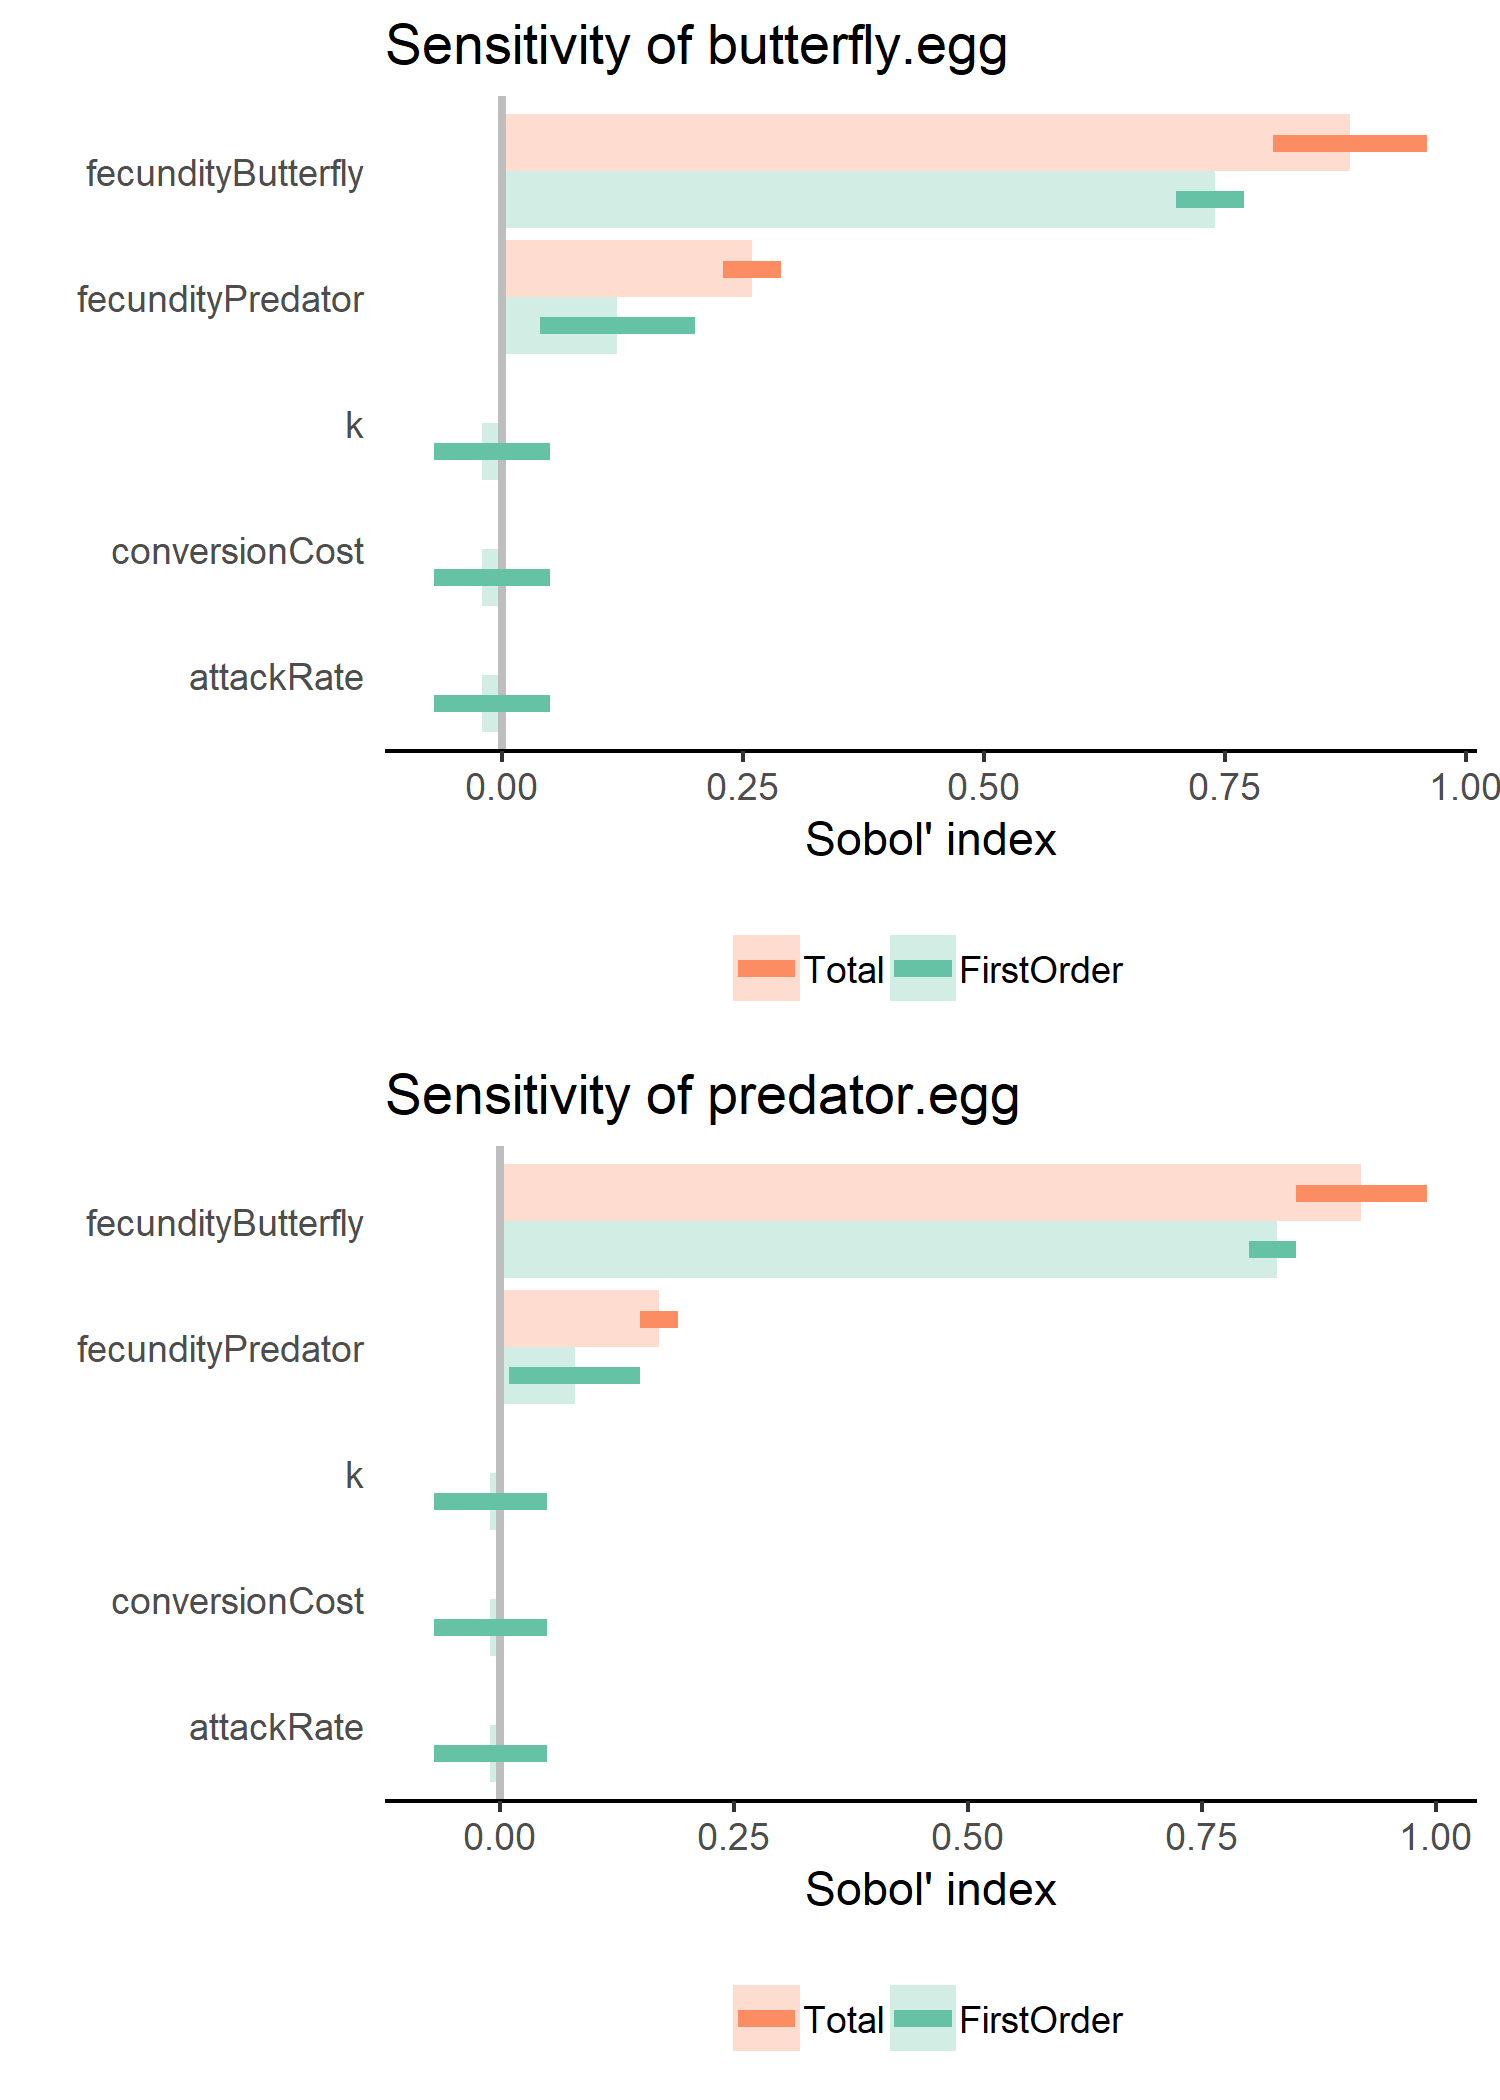
\includegraphics[width=0.7\textwidth]{graphics/sensitivity-analysis-pred-prey-3}
\caption{Sobol' indices for two model outputs and five model inputs with 95\% confidence limits. Produced by the \filename{\inputfolder/book/sensitivity-analysis-pred-prey.box} script.}
\label{fig:sensitivity-analysis-pred-prey-3}
\end{figure}

The second plot (lines 26-34) shows a bar diagram for each model output included in the analysis  (\iref{fig:sensitivity-analysis-pred-prey-3}). Each input is represented by a couple of bars, one for the first order index ($S_i$) and one for the total index ($S_{Ti}$). The narrow bars show the 95\% confidence interval, delimited by the 2.5\% and 97.5\% percentiles of the bootstrapped estimates (\cf\ line 9 in the script above).

The first order index expresses how much the variance in the model output could be reduced by fixing that input. From \iref{fig:sensitivity-analysis-pred-prey-3} we conclude that the fecundity of the butterfly is the most important parameter for the resulting number of eggs at the end of the year, both for the butterfly population and for the predator population. Predator fecundity plays a smaller but still significant role. Surprisingly, the attack rate is unimportant and the value of $k$ (expressing the variance in life stage durations) as well. Both are good news for the modeller because they are very difficult to estimate empirically.

The difference between each total and first order index ($S_{Ti}-S_i \geq 0$) tells you how much of the input's impact is due to interactions (synergies) with the other inputs. In this case, half of the impact of predator fecundity is due to interactions, for butterfly fecundity much less so.

When you carry out a sensitivity analysis, you should choose the distributions of inputs carefully. Just adding, say, $\pm 10\%$ to all inputs is certainly not the way to do it. You must provide an argument for each and every distribution chosen. The distributions you choose have an impact on the conclusion of the sensitivity analysis. Inputs that are very uncertain have a higher chance of being important (like attack rate in this case, which anyhow turned out to be insignicant). Inputs that are very certain stands a less chance of being important (like conversion cost in this case, which in fact did turn out to be insignicant).